%\documentclass{book}\usepackage{sjtfonts}\usepackage{includegraphics}\usepackage{alltt}\usepackage{latexsym}
%\usepackage{array}
%\begin{document}\input{defs0}%		miradefs.tex 		    June 1994

% opening and closing a quoted Miranda section

\newcommand{\mira}{\noindent\hrulefill\nopagebreak\so}
\newcommand{\arim}{\nopagebreak\st\hrulefill\\}

% backslash in the Miranda environment
% Only feasible approach is to use \verb+\+
% in line!

%\newcommand{\bs}{$\mi\backslash\!\!$}
%\newcommand{\lbs}{\mbox{\verb+\+}}

% ignoring part of the input

\newcommand{\ignore}[1]{}

% a blank line in a Miranda section

\newcommand{\bl}{\mbox{\ }}

% Signalling a diffculty.

\definecolor{light-gray}{gray}{0.95}

\newcommand{\beware}[2]
 {\medskip\noindent\colorbox{light-gray}{\parbox{\textwidth}
 {\mbox{\large\textbf{#1}} \medskip\noindent\\ #2}\medskip\noindent}}

% Subscripting in Miranda text
\newcommand{\subscr}[2]{\mbox{${\mbox{\texttt{#1}}}_{\mbox{\texttt{#2}}}$}}

%\newcommand{\subscr}[2]{\mbox{${\mbox{\mi #1}}_{\mbox{\smtt #2}}$}}
\newcommand{\aone}{\subscr{a}{1}}
\newcommand{\atwo}{\subscr{a}{2}}
\newcommand{\ak}{\subscr{a}{k}}

\newcommand{\aoneone}{\subscr{a}{1,1}}

\newcommand{\eone}{\subscr{e}{1}}
\newcommand{\etwo}{\subscr{e}{2}}
\newcommand{\ei}{\subscr{e}{i}}
\newcommand{\er}{\subscr{e}{r}}

\newcommand{\fone}{\subscr{f}{1}}
\newcommand{\fl}{\subscr{f}{l}}

\newcommand{\gone}{\subscr{g}{1}}
\newcommand{\gtwo}{\subscr{g}{2}}
\newcommand{\gi}{\subscr{g}{i}}
\newcommand{\gr}{\subscr{g}{r}}

\newcommand{\hone}{\subscr{h}{1}}
\newcommand{\hl}{\subscr{h}{l}}

\newcommand{\pone}{\subscr{p}{1}}
\newcommand{\ptwo}{\subscr{p}{2}}
\newcommand{\pk}{\subscr{p}{k}}

\newcommand{\qone}{\subscr{q}{1}}
\newcommand{\qtwo}{\subscr{q}{2}}
\newcommand{\qk}{\subscr{q}{k}}

\newcommand{\rone}{\subscr{r}{1}}
\newcommand{\rtwo}{\subscr{r}{2}}

\newcommand{\tone}{\subscr{t}{1}}
\newcommand{\ttwo}{\subscr{t}{2}}
\newcommand{\tn}{\subscr{t}{n}}

\newcommand{\vone}{\subscr{v}{1}}
\newcommand{\vtwo}{\subscr{v}{2}}
\newcommand{\vn}{\subscr{v}{n}}

% for regular expressions

\newcommand{\stone}{\subscr{st}{1}}
\newcommand{\sttwo}{\subscr{st}{2}}
\newcommand{\stn}{\subscr{st}{n}}
\newcommand{\rthree}{\subscr{r}{3}}

\newcommand{\eps}{$\varepsilon$}
\newcommand{\trans}[1]{\stackrel{\mbox{\tt #1}}{\longrightarrow}}



% superscript in Miranda text

\newcommand{\superscr}[2]{\mbox{${\mbox{\mi #1}}^{\mbox{\smtt #2}}$}}

% Not equals in Miranda text

\newcommand{\noteq}{\makebox[0pt][l]{=}/}
\newcommand{\overslash}{\makebox[0pt][l]{/}}

% Definitions in complexity chapter

\newfont{\oldSym}{cmsy10}
\newcommand{\Th}{\boldmath$\oldSym\Theta$}
\newcommand{\pow}[1]{\^{}#1}
\newcommand{\leqq}{$\leq$}
\newcommand{\geqq}{$\geq$}
\newcommand{\lll}{$\ll$}
\newcommand{\eqq}{$\equiv$}
\newcommand{\ltwo}{\subscr{log}{2}}

% Indexing

\newcommand{\minx}[1]{\index{#1@{\ttfamily{}#1}}}
\setcounter{chapter}{8}\setcounter{page}{143}

\chapter{Generalization: patterns of computation}
\chapstart
\label{patternsGen}

Software reuse is a major goal of the software industry.
One of the great strengths of modern functional programming languages
like Haskell is that we can use them to define
general functions which can be used in many different applications. The Haskell
prelude functions over lists, for instance, 
form a toolkit to which we turn again and again in a host of
situations.

We have already seen one aspect of
this generality in \textbf{polymorphism}, under which the same program can
be used over many different types. The 
prelude functions over lists introduced in Chapter \ref{tupleList} 
provide many examples of this
including \texttt{length}, \texttt{++} and \texttt{take}. 

As we said, these functions have the same effect over every argument --
\texttt{length} computes the length of a list of any type, for instance. In this
chapter we explore a second mechanism, by which we can write functions
which embody a \textbf{pattern of computation}; two examples of what we mean 
\index{pattern of computation}
follow. 
\begin{itemize}
\item {\em Transform every element of a list in some way}. We might turn every
alphabetic character into upper case, or double every number.
\item {\em Combine the elements of a list using some operator}. We could add
together the elements of a numeric list in this way, for example.
\end{itemize}
How can we write general functions which implement patterns like this? 
We need to make the transformation
or operator into a \textbf{parameter} of the general function; in other
words we need to have functions as arguments of other functions. These 
\textbf{higher-order functions} are
the topic of this chapter.
Complementing this is the ability to make functions the \textbf{results}
of functions; we look at that in the next chapter.

We begin the chapter by examining the patterns of computation
over lists which we have encountered so far, and in the remaining
sections of the chapter we show how these are realized as higher-order
Haskell functions. We also re-examine primitive recursive definitions,
and see that they generalize the process of combining the elements of a
list using an operator. 

Next we look at an example of generalization: taking a
function over \texttt{String} into a polymorphic, higher-order function.
We do this by identifying the parts of the function which make it
specific to
\texttt{String} and turning those into a parameter of the function.
The example serves as a model for how we can generalize functions in any situation and so make them applicable in many more contexts. 


We conclude by revisiting a number of the case studies we have looked at earlier, and encourage you to look at these again, bearing in mind the new patterns of computation introduced in this chapter.

\section{Patterns of computation over lists}
\label{defForms}
\index{pattern of computation!over lists|(}

Many of the definitions of list processing functions we have seen so far
fall into a small number
of different sorts. In this section we look back over the previous chapters and discuss
the patterns which emerge. These patterns are realized as Haskell functions
later in the chapter.

\subsection*{Applying to all -- mapping}
\index{mapping}

Many functions call for all of the elements of a list to be transformed in some
way -- this we call {\bf mapping}. We have seen examples of this from the first chapter, where
we noted that to flip a picture in a vertical mirror -- \texttt{flipV} -- 
we needed to \texttt{reverse} each line of the \texttt{Picture}, which is a list of lines. 

We also saw mapping in
Chapter \ref{tupleList} in our first example of a list comprehension 
which was to double every element of a list of integers. 
\begin{alltt}
doubleAll [2,3,71] = [4,6,142]\minx{doubleAll}
\end{alltt}
Other
examples include
\begin{titemize}
\item taking the second element of each pair in  a list of pairs, as we do in the library
database;
\item in the supermarket billing example, converting every item in a list of bar codes to the corresponding 
\texttt{(Name,Price)} pair;
\item formatting each \texttt{(Name,Price)} pair in a list.
\end{titemize}

\subsection*{Selecting elements -- filtering}
\index{filter}

Selecting all the elements of a list with a given property is also common.
Chapter \ref{tupleList} contains the example of the function which selects the
digits from a string
\begin{alltt}
digits "29 February 2004" = "292004"\minx{digits}
\end{alltt}
Among the other cases we have seen are
\begin{titemize}
\item select each pair which has a particular person as its first element;
\item select each pair which is {\em not\/} equal to the loan pair being
returned.
\end{titemize}

\subsection*{Combining the items -- folding}
\index{folding}

The first example of primitive recursion in Chapter \ref{defFunLists} was
\texttt{sum}, 
\minx{sum}
which computes the total
of a list of integers. The total of the list is given by 
\textbf{folding} the function \texttt{+} into the list, thus:
\begin{alltt}
sum [2,3,71] = 2+3+71
\end{alltt}
In a similar way, 
\begin{titemize}
\item\ \texttt{++} can be folded into a list of lists to concatenate
it, as is done in the definition of \texttt{concat};
\minx{concat}\minx{++}
\item\ \texttt{\&\&} can be folded into a list of Booleans to take their
conjunction: this is the prelude function \texttt{and}; 
\item\ \texttt{max} can be folded into a list of integers to give their maximum.
\end{titemize}

\subsection*{Breaking up lists}

A common pattern in the text processing example of Chapter \ref{defFunLists} 
is to take or drop items from a list while they have some property. 
A first example is
\texttt{getWord},
\begin{alltt}
getWord "cat dog" = "cat"\minx{getWord}
\end{alltt}
in which we continue to take characters while they are alphabetic.
Other examples include \texttt{dropWord}, \texttt{dropSpace} and
\texttt{getLine}. In the last of these
the property in question depends not only upon the particular list item but also on
the part of the list selected so far.

\subsection*{Combinations}

These patterns of definition are often used together. In defining 
\texttt{books} for the library database, which returns all the books on loan to a
given person, we filter out all pairs involving the person, and then take all
second components of the results. The strength of list comprehensions is that
they give this combination of mapping and filtering,\index{list comprehensions}
which fits some examples -- like the library database -- particularly well.

Other combinations of functions are also common.
\begin{titemize}
\item In the pictures case study the function \texttt{invertColour}\minx{invertColour} 
inverts the colour of every character in a \texttt{Picture} 
by inverting every line; inverting a line requires us to invert every character, 
so here we have two, 
nested, uses of mapping.
\item Formatting the item part of a supermarket bill involves processing each
item in some way, then combining the results, using \texttt{++}.
\end{titemize}

\subsection*{Primitive recursion and folding}
\index{folding!and primitive recursion}
\index{primitive recursion!and folding}

The form of many definitions is primitive recursive. Sorting by
insertion is a classic example:\index{sorting!insertion}
\begin{alltt}
iSort []     = []\minx{iSort}
iSort (x:xs) = ins x (iSort xs)
\end{alltt}
Haskell provides a mechanism to turn a prefix function\index{function!prefix} like \texttt{ins}
into an infix\index{function!infix}
version. The name is enclosed by back quotes, \texttt{`ins`}, so
\begin{alltt}
iSort (x:xs) = x `ins` (iSort xs)
\end{alltt}
and, in a given example, we have
\begin{alltt}
iSort [4,2,3] = 4 `ins` 2 `ins` 3 `ins` []
\end{alltt}
Looked at this way, the definition looks like \texttt{`ins`} folded into the
list \texttt{[4,2,3]}. We shall look at this again in Section \ref{foldPrimRec}. 

\subsection*{The last 10\%}

The different kinds of definition discussed so far have all been primitive
recursive: we were able to define the result for \texttt{(x:xs)} in terms of the
result for \texttt{xs}. It has been said that at least 90\% of all definitions of
list processing functions are primitive recursive. Some are not, however; in
Chapter \ref{defFunLists} notable examples are quicksort and the \texttt{splitLines}
function,
\begin{alltt}\minx{splitLines}
splitLines [] = []
splitLines ws
  = getLine lineLen ws
         : splitLines (dropLine lineLen ws)
\end{alltt}
For a non-empty list of words \texttt{ws}, the result \texttt{splitLines ws} is defined using
a recursive call of \texttt{splitLines} not on the tail of \texttt{ws} but on 
\texttt{(dropLine lineLen ws)}.
This form of recursion will terminate
because \texttt{(dropLine lineLen ws)} will always be shorter than \texttt{ws} itself,
at least in sensible cases where no word in the list \texttt{ws} is longer than the line
length \texttt{lineLen}.  

\index{pattern of computation!over lists|)}


\section{Higher-order functions: functions as arguments}
\label{hofs}
\index{function!higher-order}
\index{higher-order function}

A function is \textbf{higher-order} if it takes a function as an
argument or returns a function as a result, or does both. In this section we
show how a variety of functions, including some of the patterns
discussed in the last section, can be written using functions as
arguments.

\subsection*{Mapping -- the \texttt{map} function}

We can double all the elements in an integer list in two ways, either
using a list comprehension,
\begin{alltt}\minx{doubleAll}
doubleAll :: [Integer] -> [Integer]
doubleAll xs = [ 2*x | x <- xs ]
\end{alltt}
or using primitive recursion,
\begin{alltt}
doubleAll []     = []
doubleAll (x:xs) = 2*x : doubleAll xs
\end{alltt}
In both cases, we can see that the specific operation of multiplying
by two is applied to an element of the list in the expression `\texttt{2*x}'. 

Suppose that we want to modify every element of
a list by
another operation -- for instance, the function \texttt{ord} that transforms 
a \texttt{Char} into an \texttt{Int} --
we could modify one of the definitions above by replacing the `\texttt{2*x}' 
by `\texttt{fromEnum x}' to give a different definition. 

Taking this approach would mean that we would write a whole lot of
definitions which differ only in the function used to make the
transformation. Instead of doing this, we can write a {\em single\/}
definition in which the 
function becomes a \textbf{parameter} of the
definition. Our general definition will be
\begin{alltt}\index{map@\texttt{map}}
map f xs = [ f x | x <- xs ]\hfill(map.0)
\end{alltt}
or we can give an explicit primitive recursion
\begin{alltt}
map f []     = []\hfill(map.1)
map f (x:xs) = f x : map f xs\hfill(map.2)
\end{alltt}
The function to \texttt{double} all the elements of a list can now be given
by applying \texttt{map} to two things: the transformation -- \texttt{double} -- and
the list in question.
\begin{alltt}
doubleAll xs = map double xs	       
\end{alltt}
where \texttt{double x = 2*x}. In a similar way, 
the function to convert all the characters into their codes will be
\begin{alltt}\minx{convertChrs}
convertChrs :: [Char] -> [Int]
convertChrs xs = map fromEnum xs
\end{alltt}
In the \texttt{Picture} case study to flip a picture in a vertical
mirror we can write
\begin{alltt}\minx{flipV}
flipV :: Picture -> Picture
flipV xs = map reverse xs
\end{alltt}
What is the type of \texttt{map}? It takes two arguments -- the first is
a function, 
and
the second is a list -- and it returns a list. 
\begin{center}
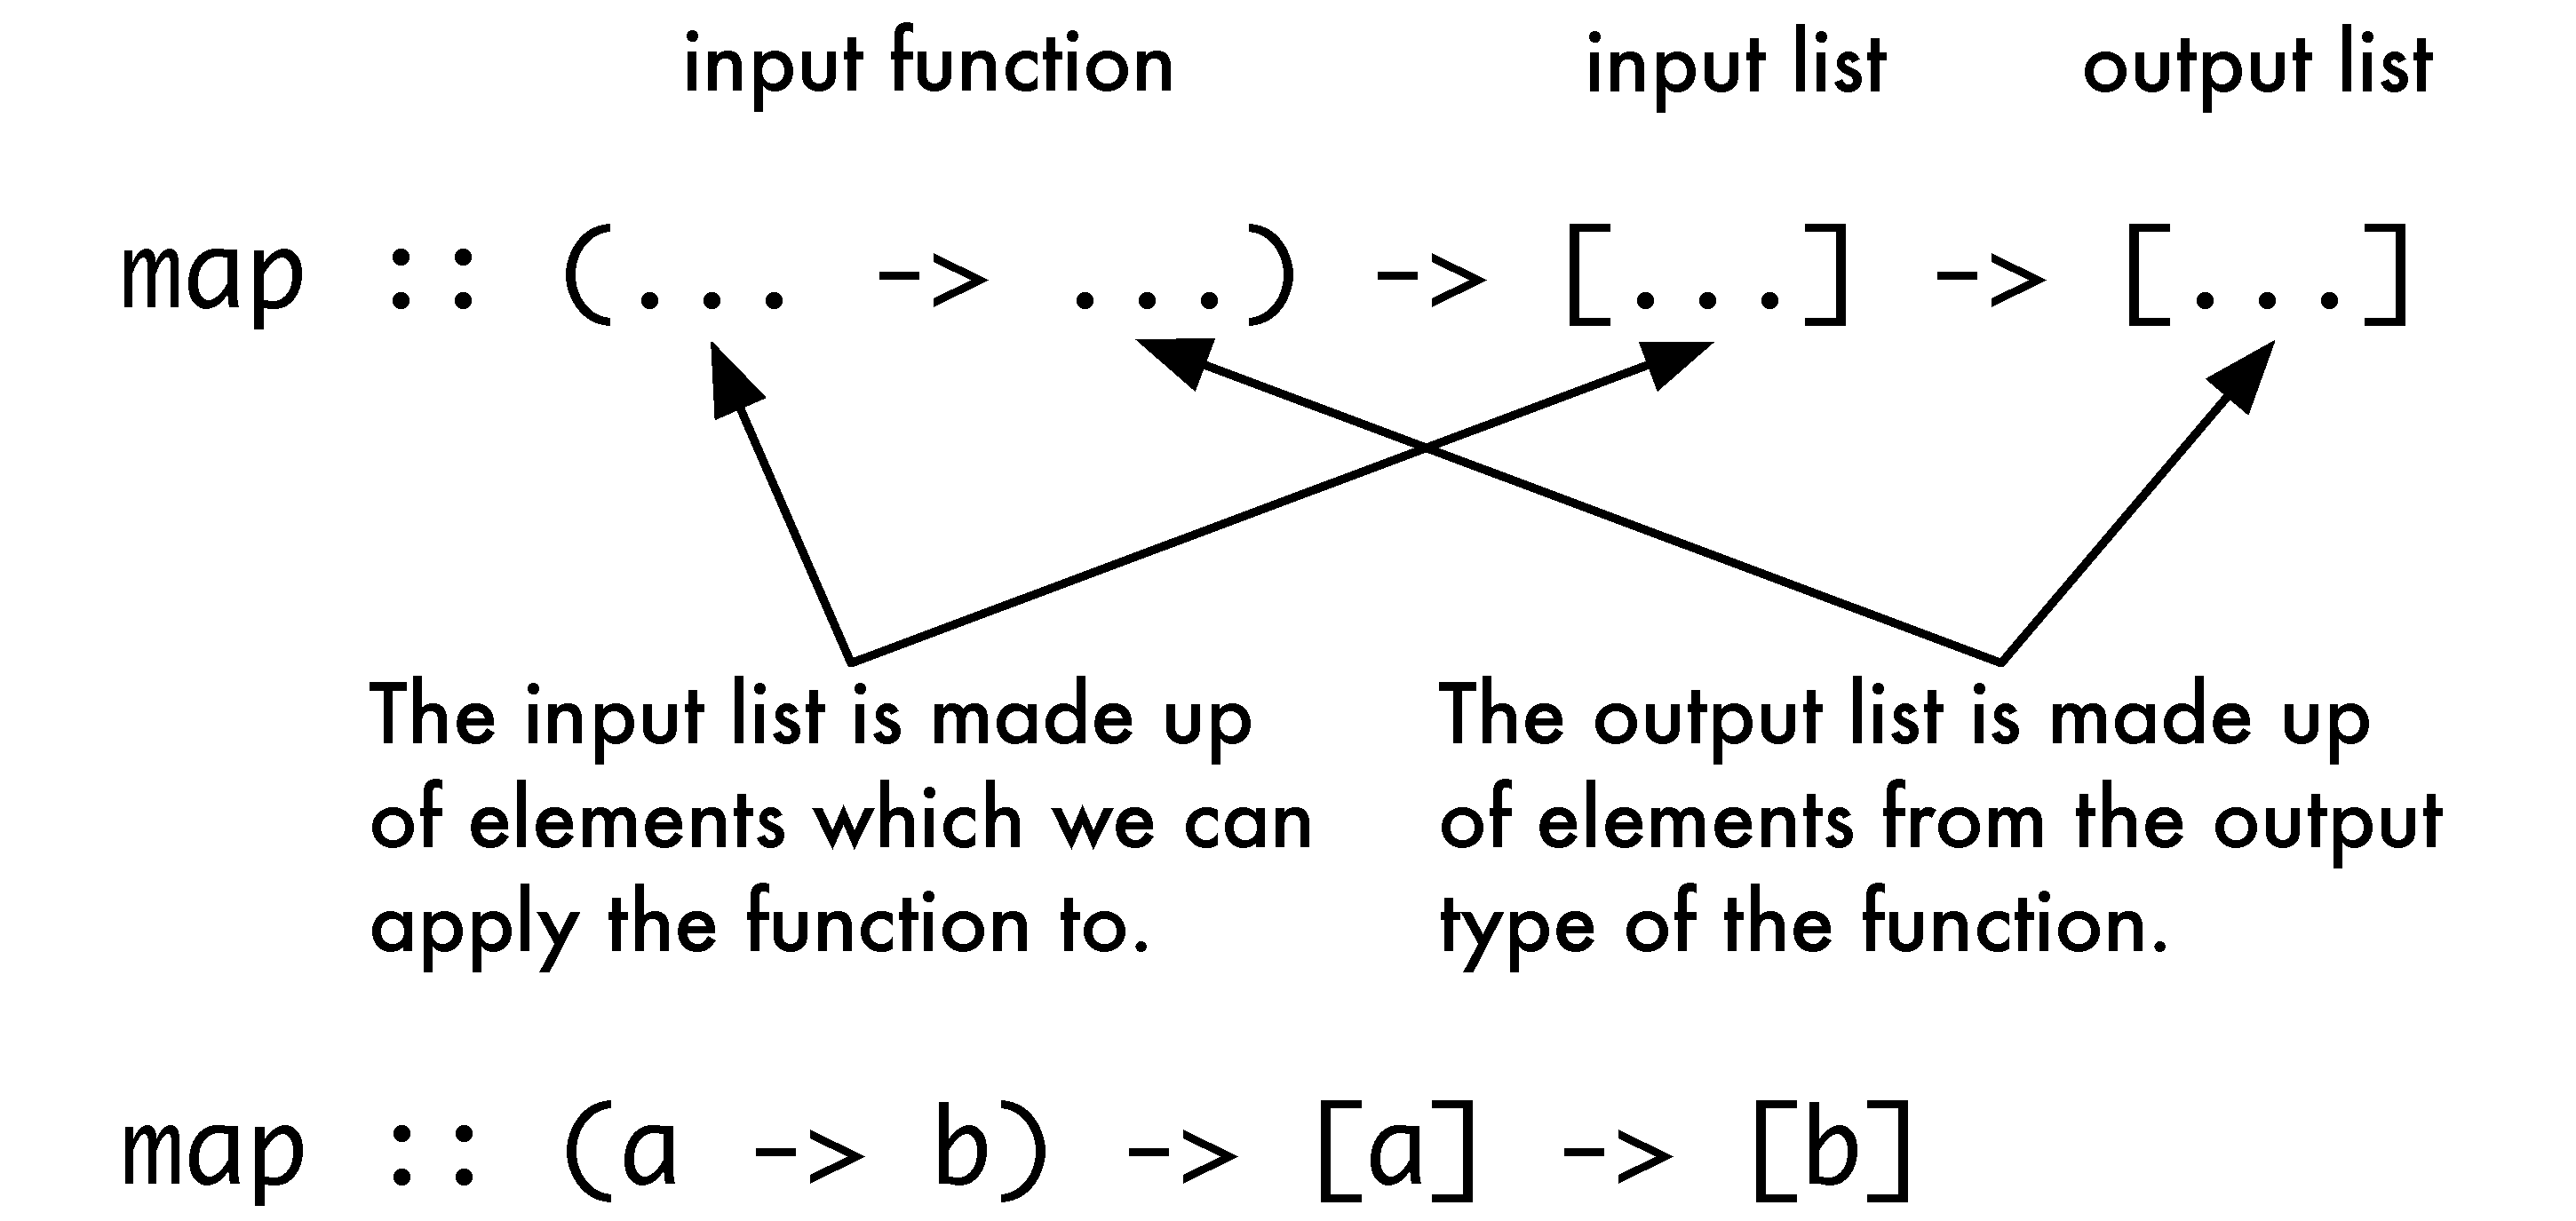
\includegraphics[width=4in]{Pictures/mapType.pdf}
\end{center}
The 
figure shows how the types of the functions and lists are related,
giving \texttt{map} the type
\begin{alltt}\index{map@\texttt{map}!type of}
map :: (a -> b) -> [a] -> [b]
\end{alltt}
where recall that \texttt{a} and \texttt{b} are type variables, standing
for arbitrary types.
Instances of the type of \texttt{map} include
\begin{alltt}
map :: (Integer -> Integer) -> [Integer] -> [Integer]
\end{alltt}
as used in the definition of \texttt{doubleAll}, where \texttt{map} is applied to
the function \texttt{double} of type \texttt{Int -> Int} and
\begin{alltt}
map :: (Char -> Int) -> [Char] -> [Int]
\end{alltt}
as in the definition of \texttt{convertChrs}.

\subsection*{Modelling properties as functions}
\index{properties as functions}
\index{function!representing properties}

Before defining the function to \textbf{filter}, or  select, 
those elements of a list having a given property, we need to think about how such
properties are to be modelled in Haskell. Take the example of filtering
the digits from a string -- the function \texttt{digits}
mentioned earlier. How is the property of `being a digit' to be
modelled? We have already seen that the library \texttt{Data.Char} contains a function
\begin{alltt}\minx{isDigit}
isDigit :: Char -> Bool
\end{alltt}
and we find out whether a particular character like \texttt{'d'} is a
digit or not by applying the function to the character to give a
Boolean result, that is \texttt{True}
or \texttt{False}.

This is the way that we can model a \textbf{property}\index{property}
over any type \texttt{t}.
The property is given by a function of type
\begin{alltt}
t -> Bool 
\end{alltt}
and an element
\texttt{x} has the property precisely when \texttt{f x} has the value
\texttt{True}. We have already seen the example of \texttt{isDigit};
other examples include
\begin{alltt}\minx{isEven}\minx{isSorted}
isEven :: Integer -> Bool
isEven n = (n `mod` 2 == 0)

isSorted :: [Integer] -> Bool
isSorted xs = (xs == iSort xs)
\end{alltt}
We usually adopt the convention that the names of properties begin with `\texttt{is}'.
\index{conventions!names of properties}

\subsection*{Filtering -- the \texttt{filter} function}
\index{filter@\texttt{filter}}

Building on our discussion of properties, we see that the \texttt{filter}
function will take a property and a list, and return those elements of
the list having the property:
\begin{alltt}
filter p [] = []\hfill(filter.1)
filter p (x:xs)
  | p x         = x : filter p xs\hfill(filter.2)
  | otherwise   =     filter p xs\hfill(filter.3)
\end{alltt}
In the case of an empty list, the result is empty.
For a non-empty list
\texttt{(x:xs)} there are two cases. If the guard condition \texttt{p x} is
true then the element \texttt{x} is the first element of the result list; the remainder
of the result is given by selecting those elements in \texttt{xs} which have the property 
\texttt{p}. If \texttt{p x} is \texttt{False}, \texttt{x} is not included, and the result is
given by searching \texttt{xs} for elements with 
property \texttt{p}.

A list comprehension also serves to define \texttt{filter},
\begin{alltt}
filter p xs = [ x | x <- xs , p x ]\hfill(filter.0)
\end{alltt}
where again we see that the condition for inclusion of \texttt{x} in the list is
that it has the property \texttt{p}.

Our example \texttt{digits}
is defined using \texttt{filter} as follows
\begin{alltt}\minx{digits}
digits xs = filter isDigit xs
\end{alltt}
Other applications of \texttt{filter} give
\begin{alltt}
filter isEven [2,3,4,5]                    \step [2,4]
filter isSorted [[2,3,4,5],[3,2,5],[],[3]] \step [[2,3,4,5],[],[3]]
\end{alltt}

What is the type of \texttt{filter}? It takes a property and a list, and
returns a list.
\begin{center}\index{filter@\texttt{filter}!type of}
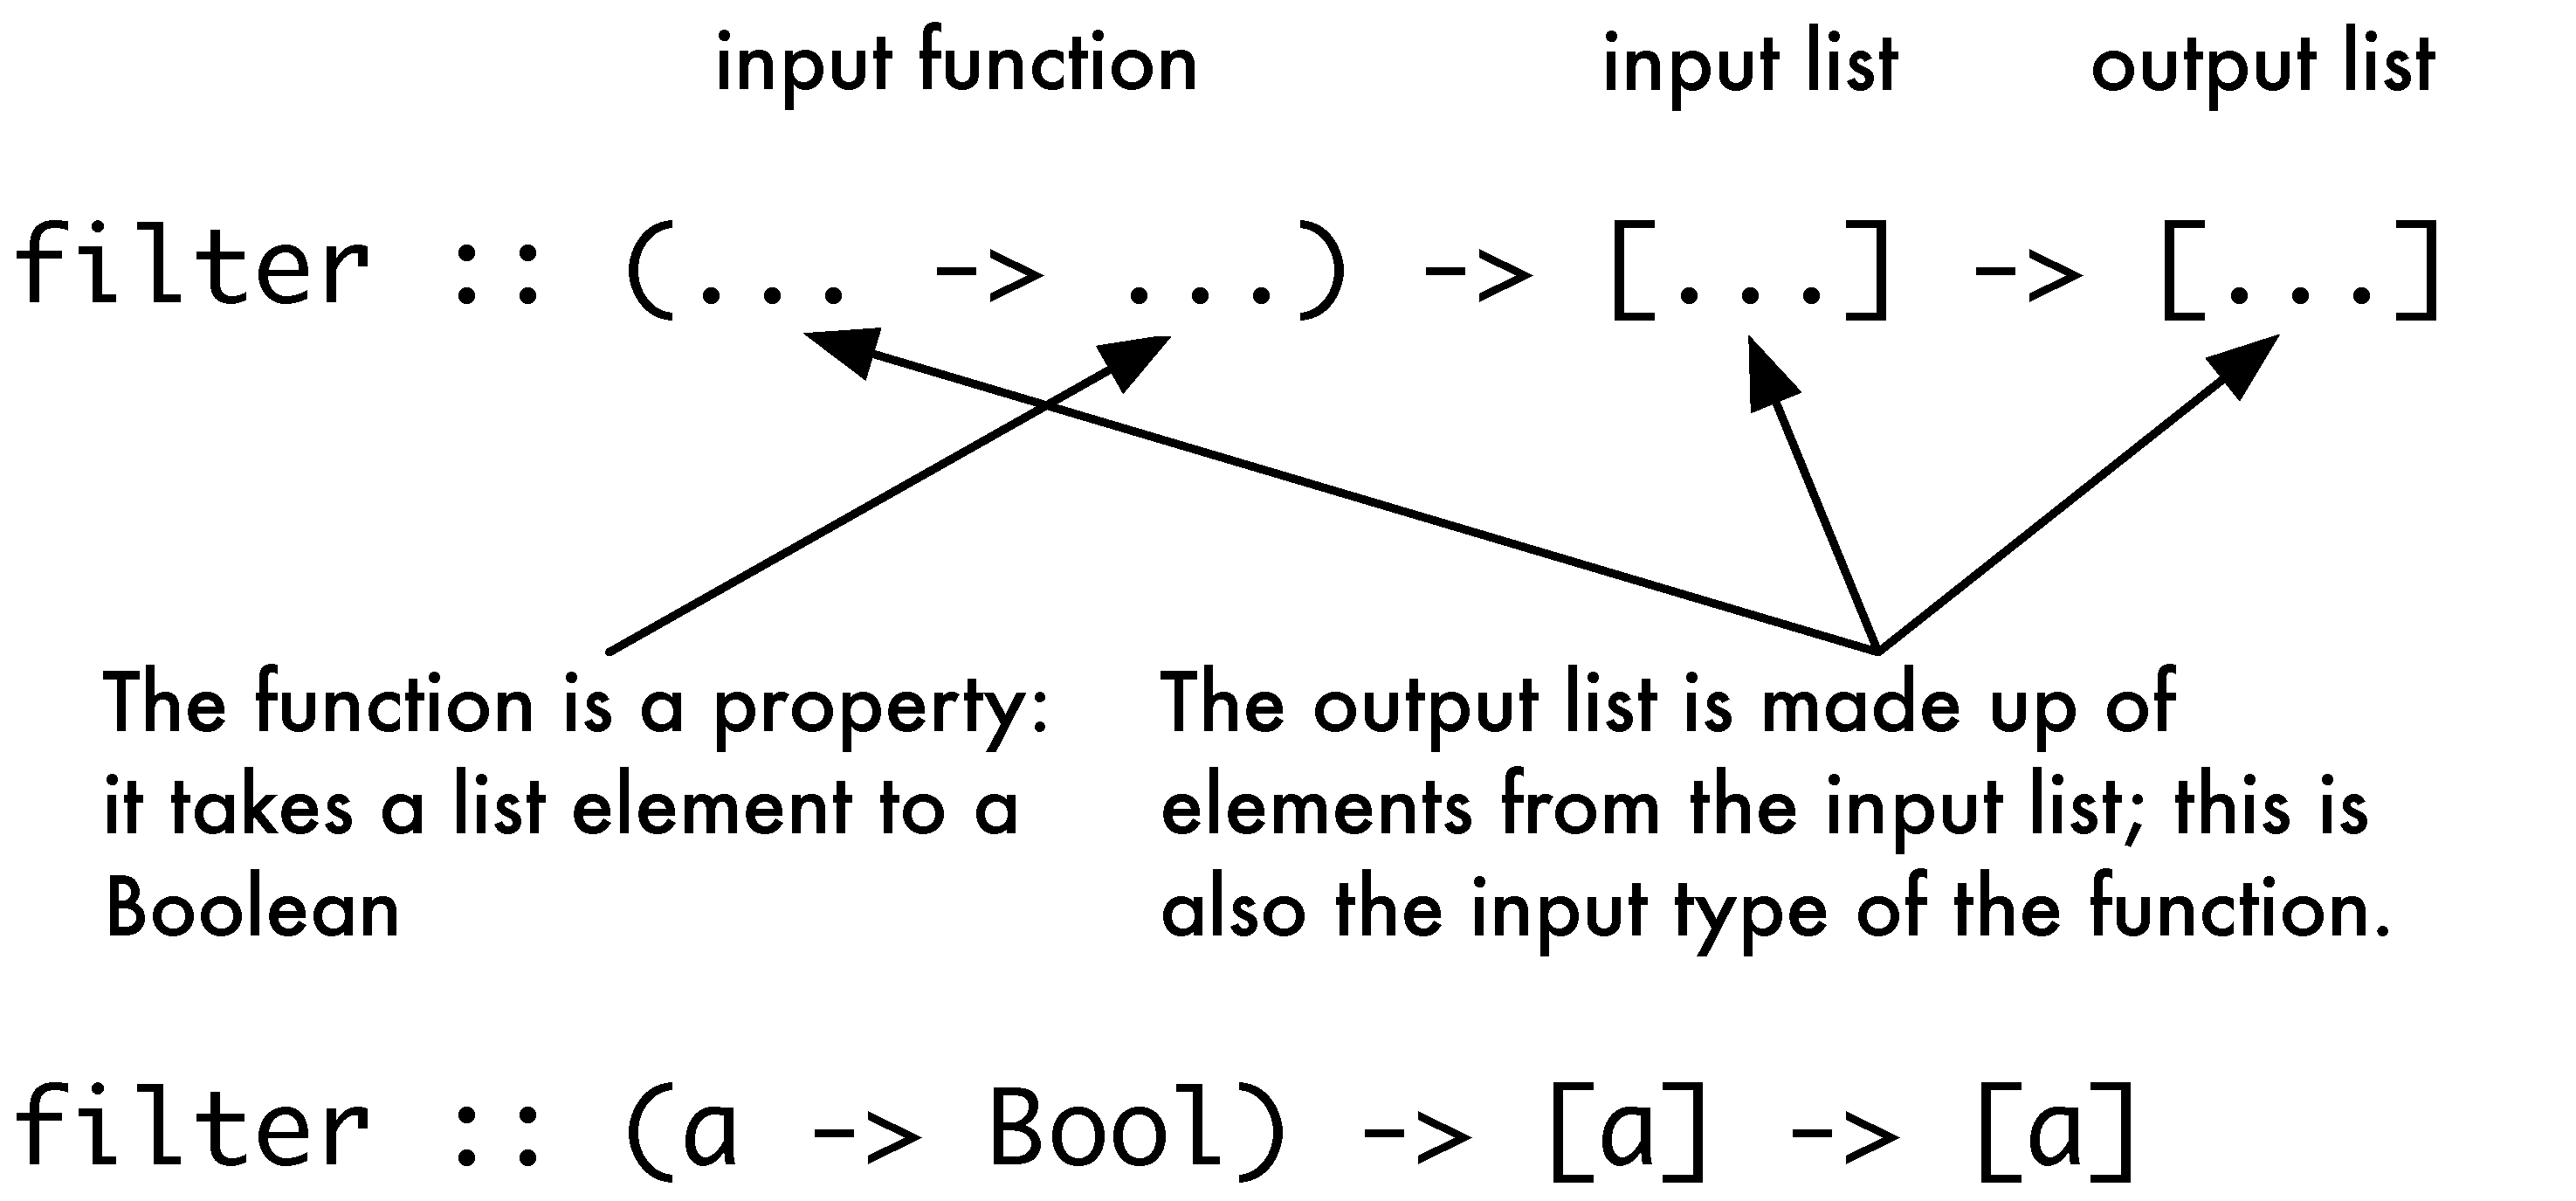
\includegraphics[width=4in]{Pictures/filterType.pdf}
\end{center}

\subsection*{Combining \texttt{zip} and \texttt{map} -- the
\texttt{zipWith} function}\index{zipWith@\texttt{zipWith}}

We have already seen the polymorphic function
\begin{alltt}
zip :: [a] -> [b] -> [(a,b)]
\end{alltt}
which `zips together' the the elements of two lists into a single list of pairs, pairing up corresponding elements in the two lists. For instance,
\begin{alltt}\index{Frank}
zip [2,3,4] "Frank" = [(2,'F'),(3,'r'),(4,'a')]
\end{alltt}
As the example shows, if the lists are of different lengths, we just drop the elements in the longer list with no element to pair with.

What happens if we want to do something to two corresponding elements 
other than making a
pair of them? Recall from Chapter \ref{intro} that in our \texttt{Picture}
case study to define \texttt{beside} we wanted to join
corresponding lines using (++).
To this end we define the \texttt{zipWith} function, which combines the
effect of zipping and mapping:
\begin{alltt}
zipWith f (x:xs) (y:ys) = f x y : zipWith f xs ys
zipWith f  _      _     = []
\end{alltt}
In the first case we see that if both lists are non-empty
we apply the function \texttt{f} to their heads to give the first element
of the result, and zip their tails with \texttt{f} in a similar way. In
the second case -- when at least one of the inputs is \texttt{[]} -- the
result is \texttt{[]}, just as it was in the definition of \texttt{zip}.

Returning to the \texttt{Picture} case study, we can then define
\begin{alltt}\minx{beside}
beside :: Picture -> Picture -> Picture
beside pic1 pic2 = zipWith (++) pic1 pic2
\end{alltt}
What is the type of \texttt{zipWith}?
The function takes three arguments. The second and third are lists of
arbitrary type, \texttt{[a]} and \texttt{[b]} respectively. The result is also
a list of arbitrary type, \texttt{[c]}. Now, the first argument is
applied to elements of the input lists to give an element of the output
list, so it must have type
\texttt{a -> b -> c}. Putting this together, we have
\begin{alltt}\index{zipWith@\texttt{zipWith}!type of}
zipWith :: (a -> b -> c) -> [a] -> [b] -> [c]
\end{alltt}

In the exercises we look further at the examples defined here, as well
as introducing other higher-order functions.

\begin{exercises}

\item
Write three line-by-line calculations of \texttt{doubleAll [2,1,7]} using
the three different definitions of \texttt{doubleAll} that use a list
comprehension, primitive recursion and \texttt{map}.

\item
How would you define the \texttt{length} function using \texttt{map} and
\texttt{sum}?


\item
Given the function
\begin{alltt}
addUp ns = filter greaterOne (map addOne ns)
\end{alltt}
where
\begin{alltt}
greaterOne n = n>1
addOne n     = n+1
\end{alltt}
how would you redefine it using \texttt{filter} before \texttt{map}, as
in
\begin{alltt} 
addUp ns = map fun1 (filter fun2 ns)
\end{alltt}

\item
Describe the effect of 
\begin{alltt}
map addOne (map addOne ns) 
\end{alltt}
Can you conclude anything in general about properties of
\texttt{map f (map g xs)}
where \texttt{f} and \texttt{g} are arbitrary functions?

\item
What is the effect of 
\begin{alltt}
filter greaterOne (filter lessTen ns)
\end{alltt}
where \texttt{lessTen n = n<10}? What about the general case of
\begin{alltt}
filter p (filter q xs)
\end{alltt}
where \texttt{p} and \texttt{q} are arbitrary properties?

\item
Give definitions of functions to take a list of integers, \texttt{ns}, and
\begin{titemize}
\item return the list consisting of the squares of the integers in \texttt{ns};
\item return the sum of squares of items in \texttt{ns};
\item check whether all items of the list are greater than zero.
\end{titemize}

\item
Using functions defined already wherever possible, write definitions of functions to 
\begin{titemize}
\item give the minimum value of a function \texttt{f} on inputs \texttt{0} to \texttt{n};
\item test whether the values of \texttt{f} on inputs \texttt{0} to \texttt{n} are all
equal;
\item test if all values of \texttt{f} on inputs \texttt{0} to \texttt{n} are greater
than zero, and,
\item check whether the values \texttt{f 0}, \texttt{f 1} to \texttt{f n} are in
increasing order.
\end{titemize}

\item
State the type of and define a function \texttt{twice} which takes a function from integers to integers
and an input integer, and whose output is the function applied to the input
twice. For instance, with the \texttt{double} function and \texttt{7} as input,
the result is \texttt{28}. What is the most general type of the function
you have defined?

\item
Give the type of and define a function \texttt{iter} so that
\begin{alltt}
iter n f x = f (f (f \ldots (f x)\ldots))  
\end{alltt}
where \texttt{f} occurs \texttt{n} times on the right-hand side of the equation.
For instance, we should have
\begin{alltt}
iter 3 f x = f (f (f x))
\end{alltt}
and \texttt{iter 0 f x} should return \texttt{x}.

\item
Using \texttt{iter} and \texttt{double} define a function which on input \texttt{n} 
returns $\texttt{2}^{\texttt{n}}$; remember that 
$\texttt{2}^{\texttt{n}}$ means one multiplied by two \texttt{n}
times.

\item
Define QuickCheck properties that you would expect to hold for the result of a \texttt{filter},
\begin{alltt}
filter p xs
\end{alltt}

\item
Suppose that \texttt{g} is the \emph{inverse} of \texttt{f}, so that 
\begin{alltt}
g (f x) \step{}x
f (g y) \step{}y
\end{alltt}
for all \texttt{x} and \texttt{y}, give properties that you would expect to hold for the result of the \texttt{map}:
\begin{alltt}
map f xs
\end{alltt}

\end{exercises}

\section{Folding and primitive recursion}
\label{foldPrimRec}
\index{folding!and primitive recursion|(}
\index{primitive recursion!and folding|(}


In this section we look at a particular sort of higher-order function
which implements the operation of \textbf{folding} an operator or function into a
list of values. We will see that this operation is more general than we
might first think, and that most primitive recursive functions over
lists can, in fact, be defined using a fold.

\subsection*{The functions \texttt{foldr1} and \texttt{foldr}}
\index{folding}
\index{foldr1@\texttt{foldr1}}\index{foldr@\texttt{foldr}}

Here we look at two sorts of folding function. First
we look at a function which folds a function into a non-empty list; it is defined in
\texttt{GHC.List} and is called \texttt{foldr1}; we will discuss why it is 
called this later in the section.

The definition of \texttt{foldr1}\index{foldr1@\texttt{foldr1}} will have two cases. 
Folding \texttt{f} into the singleton list \texttt{[a]} gives \texttt{a}.
Folding \texttt{f} into a longer list is given by 
\begin{alltt}
foldr1 f [\eone,\etwo,\ldots,\subscr{e}{k}]
  = \eone `f` (\etwo `f` ( \ldots `f` \subscr{e}{k})\ldots)
  = \eone `f` (foldr1 f [\etwo,\ldots,\subscr{e}{k}])
  = f \eone (foldr1 f [\etwo,\ldots,\subscr{e}{k}])
\end{alltt}
The Haskell definition is therefore
\begin{alltt}
foldr1 f [x]    = x\hfill(foldr1.1)
foldr1 f (x:xs) = f x (foldr1 f xs)\hfill(foldr1.2)
\end{alltt}
and the type of \texttt{foldr1} will be given by
\begin{alltt}\index{foldr1@\texttt{foldr1}!type of}
foldr1 :: (a -> a -> a) -> [a] -> a
\end{alltt}
The type shows that \texttt{foldr1} has two arguments.
\begin{itemize}
\item The first argument is a binary function over the type \texttt{a}; for
example, the function \texttt{(+)} over \texttt{Int}.
\item The second is a list of elements of type \texttt{a} which are to
be combined using the operator; for instance, \texttt{[3,98,1]}
\end{itemize}
The result is a single value of type \texttt{a}; in the running example we
have 
\begin{alltt}
foldr1 (+) [3,98,1] = 102
\end{alltt}
Other examples which use \texttt{foldr1} include
\begin{alltt}
foldr1 (||) [False,True,False] = True
foldr1 (++) ["Freak ", "Out" , "", "!"] = "Freak Out!"
foldr1 min [6] = 6
foldr1 (*) [1 ..\ 6] = 720
\end{alltt}
The function \texttt{foldr1} gives an error when applied to an empty list argument.

We can modify the
definition to give an extra argument which is the value returned on the empty list, so giving 
a function defined on all finite lists. This
function is called \texttt{foldr} 
and
is defined as follows
\begin{alltt}\index{foldr@\texttt{foldr}}
foldr f s []     = s\hfill(foldr.1)\index{foldr@\texttt{foldr}}
foldr f s (x:xs) = f x (foldr f s xs)\hfill(foldr.2)
\end{alltt}
The `\texttt{r}' in the definition is for `fold, bracketing to the \textbf{right}'.
Using this slightly more general function, whose type we predict is
\begin{center}\index{foldr@\texttt{foldr}!type of}
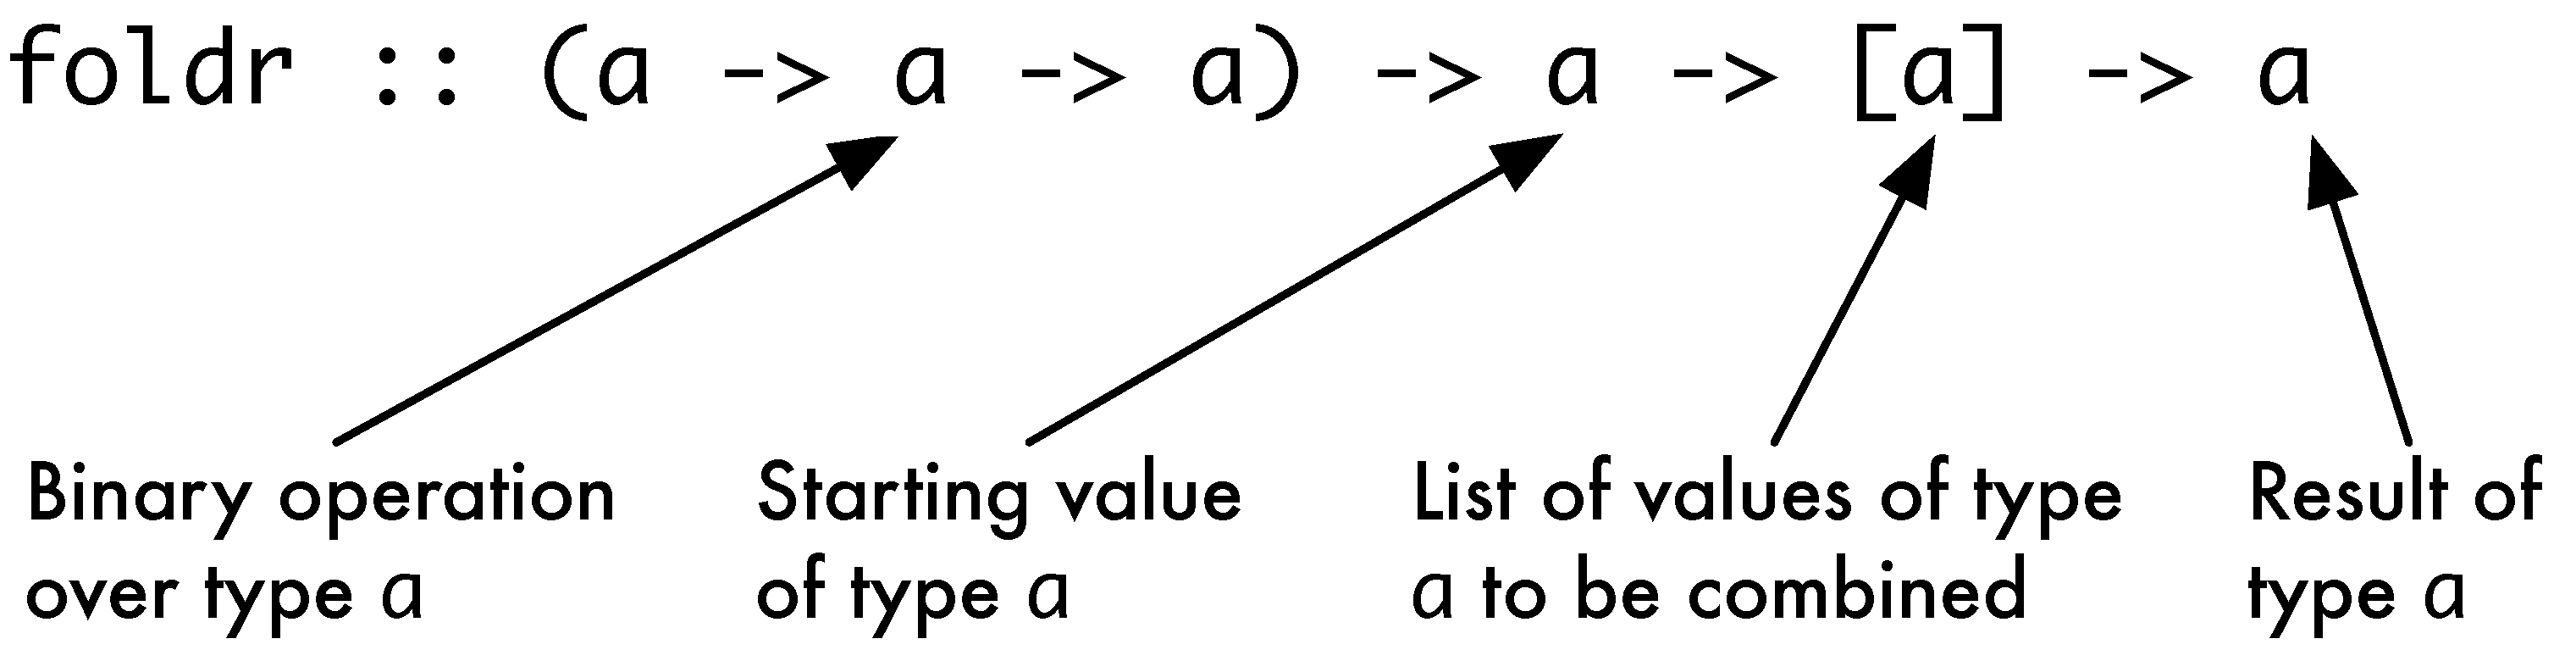
\includegraphics[width=4in]{Pictures/foldrType1.pdf}
\end{center}
we can now
define some of the standard functions of Haskell,
\begin{alltt}
concat :: [[a]] -> [a]\minx{concat}
concat xs = foldr (++) [] xs
\bl
and :: [Bool] -> Bool\minx{and}
and bs = foldr (\&\&) True bs
\end{alltt}
Returning to the start of the section, we can now see why
\texttt{foldr1} is so called: it is fold function, designed to take a
list with at least \textbf{one} element. We can also define
\texttt{foldr1} from \texttt{foldr}, like this
\begin{alltt}
foldr1 f xs = foldr f (last xs) (init xs)\hfill(foldr1.0)
\end{alltt}
where \texttt{last} gives the last element of a list, and \texttt{init} removes that element.

\subsection*{Folding in general -- \texttt{foldr} again}
\index{foldr@\texttt{foldr}}

In fact, the most general type of \texttt{foldr} is more general
than we predicted. Suppose that the starting value has type \texttt{b}
and the elements of the list are of type \texttt{a}, then
\begin{alltt}\index{foldr@\texttt{foldr}!type of}
foldr :: (a -> b -> b) -> b -> [a] -> b
\end{alltt}
We give a full explanation of how this type is derived in Section \ref{polyTypeCheck}.

With this insight about the type of \texttt{foldr} we can see
that \texttt{foldr} can be used to define another whole cohort of list functions.
For instance, we can reverse a list thus:
\begin{alltt}\minx{rev}
rev :: [a] -> [a]\minx{rev}
rev xs = foldr snoc [] xs
\bl
snoc :: a -> [a] -> [a]\minx{snoc}
snoc x xs = xs ++ [x]
\end{alltt}
This function is traditionally called \texttt{snoc} because it is like
`cons', \texttt{:},
in reverse.
We can also sort a list in this way
\begin{alltt}
iSort :: [Integer] -> [Integer]\minx{iSort}
iSort xs = foldr ins [] xs
\end{alltt}
Before we move on, we look for one last time at the definition of
\texttt{foldr}
\begin{alltt}
foldr f s []     = s\hfill(foldr.1)\index{foldr@\texttt{foldr}}
foldr f s (x:xs) = f x (foldr f s xs)\hfill(foldr.2)
\end{alltt}
What is the effect of \texttt{foldr f s}? We have two cases:
\begin{itemize}
\item the value at the empty list is given outright by \texttt{s};
\item the value at \texttt{(x:xs)} is defined in terms of the value at
\texttt{xs}, and \texttt{x} itself.
\end{itemize}
This is just like the definition of primitive recursion over
lists in Chapter \ref{defFunLists}.\footnote{There is an ambiguity in our original 
characterization. In defining the function \texttt{g} by primitive recursion the value of \texttt{g (x:xs)}
is defined in terms of both \texttt{x} and \texttt{xs} as well as the
value \texttt{g xs} itself; this makes
primitive recursion slightly more general than folding using \texttt{foldr}.}
Because of this it is no accident that we can define many of our
primitive recursive functions using \texttt{foldr}. It is usually mechanical to
go from a primitive recursive definition to the corresponding application of
\texttt{foldr}. 

How do the two approaches compare?
It is often easier initially to think of a function definition in recursive form and
only afterwards to transform it into an application of \texttt{foldr}.
One of the advantages of making this transformation is that we might
then recognize properties of the function by dint of its being a fold.
We look at proof for general functions like \texttt{map}, \texttt{filter} 
and \texttt{foldr} in Section \ref{verifGen} and we look at other fold functions in 
Chapter \ref{behaviour}.

\begin{exercises}

\item
How would you define the sum of the squares of the natural numbers \texttt{1} to
\texttt{n} using \texttt{map} and \texttt{foldr}?

\item
Define a function to give the sum of squares of the positive
integers in a list of integers.

\item
For the purposes of this exercise you should use \texttt{foldr} to
give definitions of the prelude functions
\texttt{unZip}, \texttt{last} and \texttt{init}, where examples of the
latter two
are given by\index{Peccary, Greggery}
\begin{alltt}
last "Greggery Peccary" = 'y'
init "Greggery Peccary" = "Greggery Peccar"
\end{alltt}


\item
How does the function
\begin{alltt}
mystery xs = foldr (++) [] (map sing xs)
\end{alltt}
behave, where \texttt{sing x = [x]} for all \texttt{x}?

\item
The function \texttt{formatLines} is intended to format a list of lines using the function
\begin{alltt}
formatLine :: Line -> String
\end{alltt}
to format each line in the list. Define a function 
\begin{alltt}
formatList :: (a -> String) -> [a] -> String
\end{alltt}
which takes as a parameter a function of type
\begin{alltt}
a -> String
\end{alltt}
to format each item of the list which is passed as the second parameter. Show
how \texttt{formatLines} can be defined using \texttt{formatList} and
\texttt{formatLine}.


\item
Define a function
\begin{alltt}
filterFirst :: (a -> Bool) -> [a] -> [a]
\end{alltt}
so that \texttt{filterFirst p xs} removes the first element of \texttt{xs} which does
not have the property \texttt{p}. Use this to give a version of \texttt{returnLoan}
which returns only one copy of a book. What does your function do on a list
all of whose elements have property \texttt{p}? 

\item
Can you define a function
\begin{alltt}
filterLast :: (a -> Bool) -> [a] -> [a]
\end{alltt}
which removes the last occurrence of an element of a list without property
\texttt{p}? How could you define it using \texttt{filterFirst}?



\item
How could you define a function \texttt{switchMap} which maps two functions along a list, alternating which to apply. For example,
\begin{alltt}
switchMap addOne addTen [1,2,3,4] \step{}[2,12,4,14]
\end{alltt}
where \texttt{addOne} and \texttt{addTen} behave as you would expect.
What is the most general type of \texttt{switchMap}?

\item
Define functions 
\begin{alltt}
split :: [a] -> ([a],[a])
merge :: ([a],[a]) -> [a]
\end{alltt}
so that \texttt{spilt} will split a list into two lists, picking elements alternately, while merge will interleave the two lists; for example,
\begin{alltt}
split [1,2,3,4,5] \step{}([1,3,5],[2,4])
merge ([1,3,5],[2,4]) \step{}[1,2,3,4,5]
\end{alltt}

\item
Can you formulate QuickCheck properties which characterise the way that \texttt{split} and \texttt{merge} work together?

\item {[Harder]}
Suppose that the function \texttt{g} is \emph{associative}, that is
\begin{alltt}
g x (g y z) = g (g x y) z
\end{alltt}
give a QuickCheck property that you would expect \texttt{foldr1 g (xs ++ ys)} to have. Can you think of a similar property for \texttt{foldr g s (xs ++ ys)}? Hint: you will need to think about what property \texttt{s} needs to obey.



\index{folding!and primitive recursion|)}
\index{primitive recursion!and folding|)}
\end{exercises}


\section{Generalizing: splitting up lists}
\index{generalization|(}
\index{text processing!splitting into words}

As a final example in this chapter we look at how we can generalize the
function \texttt{getWord} into a polymorphic, higher-order function.
This serves as a model for similar generalizations in many different
circumstances.

Many list manipulating programs involve splitting up lists in some way, as a
part of their processing. One way of doing this is to select some or all the
elements with a particular property -- this we have seen with \texttt{filter}.
Other ways of processing include taking or dropping elements of the list from
the front -- this we saw in the text processing example. If we know the
number of elements to be dropped, we can use
\begin{alltt}
take, drop :: Int -> [a] -> [a]\minx{take}\minx{drop}
\end{alltt}
where \texttt{take n xs} and \texttt{drop n xs} are intended to take or drop \texttt{n}
elements from the front of the list \texttt{xs}. These functions are defined in
Chapter \ref{defFunLists}.

Also in Chapter \ref{defFunLists} we looked at the example of text processing, in which
lists were split to yield words and lines. The functions 
\texttt{getWord} and \texttt{dropWord} defined there were {\em not\/} polymorphic, as they
were designed to split at whitespace characters. 

It is a general principle of functional programming that programs can often
be rewritten to use more general polymorphic and/or higher-order functions,
and we illustrate that here. 

The function \texttt{getWord} was originally defined thus:
\begin{alltt}
getWord :: String -> String\minx{getWord}
getWord []    = [] \hfill(getWord.1)
getWord (x:xs) 
  | elem x whitespace   = []\hfill(getWord.2)
  | otherwise           = x : getWord xs \hfill(getWord.3)
\end{alltt}
What forces this to work over strings is the test in \texttt{(getWord.2)}, where 
\texttt{x}
is checked for membership of \texttt{whitespace}. We can generalize the
function to have the test -- or property -- as a parameter. 

How is this to be done? Recall that a property over the type \texttt{a} is
represented by a function of type \texttt{(a -> Bool)}. Making this test a
parameter we have
\begin{alltt}
getUntil :: (a -> Bool) -> [a] -> [a]\minx{getUntil}
getUntil p []    = [] 
getUntil p (x:xs) 
  | p x         = []
  | otherwise   = x : getUntil p xs
\end{alltt}
in which the test \texttt{elem x whitespace} has been replaced by the test 
\texttt{p x}, the arbitrary property \texttt{p} applied to \texttt{x}. We can of course
recover \texttt{getWord} from this definition: 
\begin{alltt}
getWord xs 
  = getUntil p xs
    where 
    p x = elem x whitespace
\end{alltt}
\ignore{
Anticipating the next chapter a little, we can in fact write,
\begin{alltt}
getWord = getUntil (\bs{x} -> elem x whitespace)
\end{alltt}
} % end ignore
Built into Haskell are the functions \texttt{takeWhile}\minx{takeWhile}
and \texttt{dropWhile}\minx{dropWhile},
which are like \texttt{getUntil} and \texttt{dropUntil}, except that
they take or drop
elements while the condition is \texttt{True}. For instance,
\begin{alltt}
takeWhile :: (a -> Bool) -> [a] -> [a]
takeWhile p []    = [] 
takeWhile p (x:xs) 
  | p x         = x : takeWhile p xs
  | otherwise   = []
\end{alltt}
\texttt{getUntil} can be defined using \texttt{takeWhile}, and vice versa.

\index{generalization|)}


\begin{exercises}

\item
Give the type and definition of the generalization \texttt{dropUntil} of the function
\texttt{dropWord}.

\item
How would you define the function \texttt{dropSpace} using \texttt{dropUntil}?
How would you define \texttt{takeWhile}
using \texttt{getUntil}?

\item
How would you split a string into lines using \texttt{getUntil} and \texttt{dropUntil}?

\item
The function \texttt{getLine} of Chapter \ref{defFunLists} has a polymorphic type --
what is it? How could you generalize the test in this function? If you do
this, does the type of the function become more general? Explain your
answer.

\item
Can you give generalizations to polymorphic higher-order functions of the 
text processing functions \texttt{getLine}, \texttt{dropLine} and \texttt{splitLines}? 
\end{exercises}



\section{Case studies revisited}

We have already seen how the functions introduced here, \texttt{map}, \texttt{filter} and \texttt{zipWith} and so forth, can be used to re-define many of the functions from the pictures case study. This section goes back to look at other examples from that case study, as well as at others.

\subsection*{Pictures}\index{pictures}

We have discussed the \texttt{Picture} type and the functions over it already in Chapter \ref{intro}, Sections \ref{picModuleEx} and \ref{localDefs} and Chapter \ref{progLists}. In this chapter we have seen that we can define \texttt{flipV} using \texttt{map}, and \texttt{beside} using \texttt{zipWith}. The exercises that follow pick up other examples.

\begin{exercises}

\item
How can you use \texttt{map} to define the \texttt{invertColour} function, which turns a Picture into its negative?

\item
How can you use \texttt{zipWith} to define the \texttt{superimpose} function, 
\begin{alltt}
superimpose :: Picture -> Picture -> Picture
\end{alltt}
which superimposes one \texttt{Picture} (the first argument) on top of another (the second)? What does your function do if the pictures are not the same size? Can you modify your definition so that it handles this case properly?

\item {[Harder]}
Using \texttt{map} and any other functions that you need, define the function
\begin{alltt}
rotate90 :: Picture -> Picture
\end{alltt}
which rotates a picture through 90 degrees. 



\end{exercises}

\subsection*{Library database and supermarket billing}\index{library database}\index{supermarket billing}

In the database and supermarket billing examples, Sections \ref{library} and \ref{superBill}, we used list comprehensions heavily. Clearly we could have instead used \texttt{map},  \texttt{filter} and other standard list functions such as \texttt{sum}. It is a useful exercise to revisit these examples and to try re-defining some of the functions. 


\begin{exercises}

\item
Re-implement the functions
\begin{alltt}
books       :: Database -> Person -> [Book]
borrowers   :: Database -> Book -> [Person]
borrowed    :: Database -> Book -> Bool
numBorrowed :: Database -> Person -> Int
makeLoan   :: Database -> Person -> Book -> Database
returnLoan :: Database -> Person -> Book -> Database
\end{alltt}
using the functions \texttt{map},  \texttt{filter} and so on.

\item
Re-implement the functions from the previous exercise using this new definition of the 
\texttt{Database} type:
\begin{alltt}
type Database = [(Person,[Book])]
\end{alltt}

\item
Revisit the exercises of Section \ref{superBill}, where the supermarket billing example was developed, and re-implement your solutions using the prelude and library functions \texttt{map},  \texttt{filter} and so on.

\item
In the light of the previous exercises, can you come to any conclusions about when it is sensible to use list comprehensions, and when it is more useful to use the prelude and library functions explicitly?



\end{exercises}

\subsection*{Rock - Paper - Scissors}\index{Rock - Paper - Scissors}

We introduced the Rock - Paper - Scissors game in Section \ref{EnumTypes} and built on that by defining strategies in Section \ref{strategiesRPS} and showing how to play the game interactively in Section \ref{playingRPS}. 


\begin{exercises}

\item
Using the function \texttt{outcome} from Exercise 8.1 (page \pageref{outcome})
and standard list functions such as \texttt{map}, redefine the function
\begin{alltt}
tournamentOutcome :: Tournament -> Integer
\end{alltt}
described in Exercise 8.2.

\item
Redefine the function
\begin{alltt}
showTournament :: Tournament -> String
\end{alltt}
first introduced on page \pageref{showTournament}, using the standard list functions introduced in this chapter.



\end{exercises} 



\begin{summary}
This chapter has shown how the informal patterns of definition over
lists can be realized as higher-order, polymorphic functions, such as
\texttt{map}, \texttt{filter} and \texttt{foldr}. We saw how these
functions arose, and also how their types were derived, as well as
reviewing the ways in which they could be used to solve problems.

Next we looked at an example of how to generalize a function -- the
particular example was taken from the text processing case study, but
the example serves as a model for how to generalize functions in
general. The chapter concludes with a re-examination of some of the case studies.

The chapter has focused on how to write functions which take other
functions as arguments; where do these arguments come from? One answer
is that they are already defined; another is that they come themselves
as the results of Haskell functions -- this is the topic of the next
chapter.

\end{summary}


%\end{document}
